% QUANTICS 2026 submission -- Springer LNCS format
% Build:  pdflatex paper && bibtex paper && pdflatex paper && pdflatex paper
% (requires llncs.cls and splncs04.bst, shipped alongside this file)
\documentclass[runningheads]{llncs}

\usepackage[T1]{fontenc}
\usepackage{graphicx}
\usepackage{amsmath}
\usepackage{amssymb}
\usepackage{mathtools}
\usepackage{booktabs}
\usepackage{xcolor}
\usepackage{algorithm}
\usepackage{algpseudocode}
\usepackage{hyperref}
\renewcommand\UrlFont{\color{blue}\rmfamily}
\urlstyle{rm}

\graphicspath{{figures/}}

\begin{document}

\title{Learning When to Stop: Deep Reinforcement Learning\\ for Adaptive Shot Allocation in Quantum Circuit Execution}
\titlerunning{DRL for Adaptive Shot Allocation in Quantum Circuits}

\author{Sergio De Crescenzo \and
Giuseppe Bisicchia\orcidID{0000-0003-2384-2480} \and
Alessandro Bocci\orcidID{0000-0002-7649-3013} \and
Antonio Brogi\orcidID{0000-0003-2048-2098}}
\authorrunning{S. De Crescenzo et al.}

\institute{Department of Computer Science, University of Pisa, Pisa, Italy\\
\email{sergiodecrescenzo2003@gmail.com}\\
\email{\{giuseppe.bisicchia,alessandro.bocci,antonio.brogi\}@unipi.it}}

\maketitle

\begin{abstract}
Quantum algorithms are executed by repeatedly sampling a circuit -- a process
known as performing \emph{shots} -- in order to estimate its output
distribution. Choosing how many shots to run is a practical and consequential
decision: too few yield statistically unreliable results, while too many waste
scarce and costly quantum hardware time. Existing solutions either rely on
conservative a-priori concentration bounds or on hand-crafted online stopping
heuristics tailored to specific algorithm families. We investigate whether an
agent can instead \emph{learn} a stopping policy directly from execution data,
under a fully black-box assumption that makes no use of the circuit structure or
the backend noise model. We frame adaptive shot allocation as a Markov Decision
Process and train a Deep Q-Network that, at every batch of shots, observes an
eight-feature ``instrument panel'' of the running empirical distribution and
decides whether to continue or to stop. The agent is rewarded against an
a-posteriori optimal shot count derived from the point of diminishing returns.
We train and evaluate on QSimBench, using a strict split in which the 36
benchmark traces of a recent state-of-the-art study are held out and never seen
during training. The learned policy adopts a safety-first behaviour, drastically
outperforms a-priori Weissman and Hoeffding bounds, and is competitive with
purpose-built divergence-based online policies, demonstrating that black-box
shot allocation is learnable. We discuss the strengths and the current
limitations of the approach, and outline the road toward closing the remaining
gap with the best online heuristics.

\keywords{Quantum Computing \and Quantum Software Engineering \and Shot
Allocation \and Deep Reinforcement Learning \and Deep Q-Network \and NISQ.}
\end{abstract}

\section{Introduction}
\label{sec:intro}

Quantum computation is inherently probabilistic: measuring a quantum circuit
collapses its state to a single classical outcome sampled from an unknown
probability distribution determined by the circuit and the hardware
noise~\cite{nielsen2010quantum}. To obtain a meaningful estimate of that
distribution, the same circuit must be executed many times; each repetition is a
\emph{shot}, and the empirical frequencies over many shots approximate the
underlying \emph{ground truth}.

How many shots are enough? This deceptively simple question has a direct impact
on both the accuracy of the result and the cost of obtaining it. On today's
\emph{Noisy Intermediate-Scale Quantum} (NISQ) devices~\cite{preskill2018nisq},
hardware time is scarce, expensive, and shared through queued cloud access, so
every redundant shot is wasted budget. Conversely, stopping too early produces
high-variance estimates and scientifically invalid conclusions. Practitioners
typically fix the shot count up front from rules of thumb, which is either
wasteful or unreliable because the right number depends on the specific circuit
and backend.

Recent work reframed this as the \emph{point of diminishing
returns}~\cite{bisicchia2026shots}: the moment at which additional shots no
longer meaningfully change the cumulative empirical distribution of a fixed
(static, non-variational) circuit. The \textsc{IncrementalExecution} framework
operationalises this idea as an online, black-box procedure that executes shots
in batches and stops once a divergence-based stability criterion is met. While
effective, such a procedure embeds a hand-designed stopping rule whose
sensitivity must be tuned through a large grid of hyperparameters.

In this paper we ask a complementary question: \emph{can the stopping policy
itself be learned?} Rather than designing a fixed convergence test, we let a
\emph{Deep Reinforcement Learning} (DRL) agent discover one by interacting with
simulated quantum executions and receiving feedback on the quality of its
stopping decisions. The agent operates under the same black-box assumption as
\textsc{IncrementalExecution}: it never sees the circuit structure or the noise
model, only the statistics of the outcomes observed so far.

\paragraph{Contributions.} The contributions of this work are:
\begin{enumerate}
  \item We formulate adaptive shot allocation as a Markov Decision Process and
  solve it with a Deep Q-Network (DQN) that decides, batch by batch, whether to
  continue executing or to stop, using only a compact black-box view of the
  running empirical distribution (Section~\ref{sec:method}).
  \item We design an eight-feature state representation -- an ``instrument
  panel'' combining static problem descriptors with dynamic convergence signals
  -- and an asymmetric reward that encodes the domain-specific asymmetry between
  under- and over-sampling (Section~\ref{sec:method}).
  \item We train and evaluate the agent on QSimBench~\cite{qsimbench} under a
  strict no-leakage split, holding out the exact 36 benchmark traces used by the
  state-of-the-art study of Bisicchia et al.~\cite{bisicchia2026shots}, and we
  compare the learned policy against five reference methods on identical traces
  (Sections~\ref{sec:setup}--\ref{sec:results}).
  \item We provide a critical analysis of the learned behaviour, showing it is
  robust and safety-oriented, vastly superior to a-priori bounds, and
  competitive with -- though not yet superior to -- the best divergence-based
  online policy (Section~\ref{sec:results}).
\end{enumerate}

\section{Background and Related Work}
\label{sec:background}

\subsection{The Shot-Allocation Problem and the Point of Diminishing Returns}

We consider \emph{static, non-variational} circuits, whose structure and
parameters are fixed across all shots, so the effective output distribution is
stationary throughout an execution. Let $P$ be the unknown distribution over the
finite set of measurement outcomes of a circuit $C$ run on a backend $Q$, and
let $\hat{P}_n$ be the empirical distribution after $n$ shots. By the law of
large numbers $\hat{P}_n \to P$ almost surely, so for a divergence
$\mathcal{D}(\cdot,\cdot)$ the deviation $\mathcal{D}(\hat{P}_n, P)$ vanishes as
$n$ grows.

Since $P$ is inaccessible on real hardware, Bisicchia et
al.~\cite{bisicchia2026shots} adopt an \emph{a-posteriori} reference: the
empirical distribution $\hat{P}_{\mathcal{B}}$ obtained under a fixed budget
$\mathcal{B}$. The a-posteriori optimal shot count is the smallest prefix length
$n^{\star}$ whose distribution is within a tolerance $\delta$ of the full-budget
reference, robustly to later fluctuations:
\begin{equation}
  n^{\star} = \min\bigl\{\, n \le \mathcal{B} \;\big|\;
  \mathcal{D}(\hat{P}_m, \hat{P}_{\mathcal{B}}) \le \delta \;\;\forall m \ge n \,\bigr\}.
  \label{eq:oracle}
\end{equation}
We use this quantity, computed by the suffix-stable Algorithm~1
of~\cite{bisicchia2026shots} with the Total Variation Distance (TVD), as our
\emph{Oracle}: the ground-truth label against which a stopping decision is
scored. Throughout, we fix $\mathcal{B}=20{,}000$ shots, a batch size of $50$,
and $\delta=0.10$.

\subsection{Existing Approaches to Shot Optimisation}

\paragraph{A-priori concentration bounds.} Hoeffding-style~\cite{hoeffding1963}
and Weissman-style~\cite{weissman2003inequalities} inequalities provide
worst-case shot counts that guarantee a target deviation with high probability.
They depend only on $\delta$, the confidence level, and the alphabet size, and
are therefore independent of the actual circuit. This makes them safe but
extremely conservative, often overestimating the required shots by several
orders of magnitude.

\paragraph{Adaptive allocation for variational algorithms.} A large body of work
dynamically reallocates shots across the iterations of variational quantum
algorithms~\cite{cerezo2021vqa,kandala2017vqe}, using gradient variance, utility
per iteration, or output entropy. These methods assume an iterative optimisation
loop with non-stationary distributions and do not transfer to the static-circuit
setting we target.

\paragraph{Learning-based methods.} Reinforcement learning has been applied to
shot scheduling within VQE optimisation, and supervised schedules have been used
in quantum machine learning~\cite{phalak2023shot}. These approaches are tied to
specific workloads and rely on task-specific supervision signals.

\paragraph{Online black-box control.} Closest to our setting is the
\textsc{IncrementalExecution} framework~\cite{bisicchia2026shots}, which detects
the point of diminishing returns online from the observed outcomes alone. Its
behaviour is governed by pluggable stopping, stability, and allocation policies;
its best configurations (denoted \mbox{Inc-TVD}, \mbox{Inc-Hell}, \mbox{Inc-JS}
according to the divergence used) constitute the strongest baselines for static
circuits. Our work keeps the same black-box assumption but replaces the
hand-crafted stopping rule with a \emph{learned} one.

\subsection{Deep Q-Networks}

Reinforcement learning models an agent interacting with an environment over
discrete steps, choosing actions to maximise a cumulative
reward~\cite{sutton2018reinforcement}. Q-learning~\cite{watkins1992qlearning}
estimates the action-value function $Q(s,a)$, the expected return of taking
action $a$ in state $s$. When the state space is large or continuous, the table
is replaced by a neural function approximator, yielding the Deep Q-Network
(DQN)~\cite{mnih2015human}, stabilised by \emph{experience replay} (training on
random mini-batches of past transitions) and a periodically synchronised
\emph{target network}. We adopt this well-established machinery as the learning
backbone.

\section{Method}
\label{sec:method}

\subsection{System Architecture}

Our learning system comprises three interacting components
(Fig.~\ref{fig:arch}). The \emph{quantum environment} is a simulated playground,
built on QSimBench, that executes batches of shots and exposes the running
statistics of the outcomes. The \emph{Oracle} is a direct implementation of the
a-posteriori optimum of Eq.~\eqref{eq:oracle}; crucially, its answer is used
\emph{only} at the end of an episode to score the agent and is never revealed
during decision making. The \emph{agent} is the DQN learner that, at each step,
observes the environment state and chooses to continue or to stop.

\begin{figure}[t]
\centering
% architecture sketch (text-based to keep the build self-contained)
\fbox{\parbox{0.92\textwidth}{\centering\small
\textbf{DQN agent (Learner)} $\;\xrightarrow{\;\text{action: continue / stop}\;}\;$
\textbf{Quantum environment (Playground)}\\[2pt]
\textbf{DQN agent} $\;\xleftarrow{\;\text{state, reward}\;}\;$
\textbf{Quantum environment}\\[4pt]
at episode termination only:\quad
\textbf{Quantum environment} $\;\xrightarrow{\;\text{query}\;}\;$
\textbf{Oracle} $\;\xrightarrow{\;\text{optimal shots}\;}\;$ \textbf{reward}\\[2pt]
(\textbf{Oracle} = a-posteriori optimum, Eq.~\eqref{eq:oracle})
}}
\caption{High-level architecture. The agent observes states and acts iteratively
until it stops. Only at episode termination does the environment consult the
Oracle to compute the reward; the Oracle's optimal shot count is never shown to
the agent during decision making.}
\label{fig:arch}
\end{figure}

\subsection{State Space}

The state $\mathbf{s}_t \in [0,1]^8$ is an ``instrument panel'' of eight
features, each normalised to aid training. Four are \emph{static} descriptors of
the problem instance and four are \emph{dynamic} signals recomputed after every
batch:
\begin{description}
  \item[Static] (i) an algorithm encoding, (ii) the circuit size (number of
  qubits), (iii) a backend encoding, and (iv) the current shot count as a
  fraction of the budget (a progress bar).
  \item[Dynamic] (v) the normalised Shannon \emph{entropy} of the cumulative
  distribution (its spread), (vi) the \emph{variance} of the outcome
  probabilities (peakedness), (vii) the \emph{rate of change}, i.e.\ the TVD
  between the cumulative distribution and the latest batch -- the agent's core
  convergence signal -- and (viii) a \emph{relative-progress} term comparing the
  current shot count to a size-dependent heuristic, which lets the agent tell
  early statistical noise from genuine late convergence.
\end{description}
The static features let the agent recognise the kind of circuit it faces, while
the dynamic features let it perceive, in real time, how close the empirical
distribution is to stabilising.

\subsection{Actions and Episode Dynamics}

The action space is binary: \textsc{continue} executes one more batch of $50$
shots and updates the state; \textsc{stop} terminates the episode. An episode
also terminates automatically if the budget $\mathcal{B}$ is exhausted. On
termination the environment compares the agent's total shot count to the Oracle's
$n^{\star}$ and emits the terminal reward.

\subsection{Reward Design}

The reward combines a small step-wise efficiency penalty with a dominant
terminal signal. Each \textsc{continue} incurs a penalty of $-0.02$, applying
gentle, continuous pressure against unnecessarily long episodes. The terminal
reward is deliberately \emph{asymmetric}, reflecting that the two failure modes
are not equally harmful: under-sampling yields statistically invalid results,
whereas over-sampling merely wastes resources. Let
$\text{error} = n_{\text{agent}} - n^{\star}$. Then
\begin{equation}
  R_{\text{term}} =
  \begin{cases}
    \bigl(-1.85 - \tfrac{|\text{error}|}{n^{\star}}\bigr)\,\sigma,
      & \text{error} < 0 \quad (\text{undershoot}),\\[4pt]
    e^{-0.00025\,\cdot\,\text{error}},
      & \text{error} \ge 0 \quad (\text{overshoot}),
  \end{cases}
  \label{eq:reward}
\end{equation}
where $\sigma = 1 + 0.5\,n^{\star}/\mathcal{B}$ scales the penalty with problem
difficulty. Overshooting decays smoothly from the maximum reward at a perfect
stop, while undershooting is treated as a categorical failure with a large
negative reward. This asymmetry instils a principled safety-first bias.

\subsection{Network and Learning Algorithm}

The action-value function is approximated by a multi-layer perceptron with input
dimension $8$, three hidden layers of $512$, $256$, and $128$ ReLU units (with
$10\%$ dropout after the first two for regularisation), and a two-unit linear
output giving $Q(s,\textsc{continue})$ and $Q(s,\textsc{stop})$. Training follows
standard DQN: an $\varepsilon$-greedy behaviour policy ($\varepsilon$ decaying
from $1.0$ to $0.05$), an experience-replay buffer of $200{,}000$ transitions,
mini-batches of $64$, the Adam optimiser at learning rate $10^{-4}$, a discount
factor $\gamma = 0.99$, and a target network synchronised every $500$ episodes.
The Bellman target is $r + (1-\text{done})\,\gamma\,\max_{a'} Q_{\text{target}}(s',a')$
and the loss is the mean squared temporal-difference error.

\subsection{Dataset, Oracle Labels, and Strict Split}
\label{sec:dataset}

We use QSimBench~\cite{qsimbench}, an execution-level benchmark providing more
than 20 million precomputed shot-level traces across many algorithms (e.g.\ dj,
qaoa, qft, vqe, qnn, random), circuit sizes from $4$ to $14$ qubits, and IBM
noisy backend simulators (\texttt{fake\_fez}, \texttt{fake\_kyiv},
\texttt{fake\_marrakesh}, \texttt{fake\_sherbrooke}, \texttt{fake\_torino}).
Each problem instance is a triplet (algorithm, size, backend); its Oracle label
$n^{\star}$ is precomputed once via Eq.~\eqref{eq:oracle}.

To enable a fair, leakage-free comparison with the state of the art, we reserve
as the \emph{test set} the exact 36 traces used in the evaluation tables
of~\cite{bisicchia2026shots} (18 small circuits with $n<10$, 18 large with
$n\ge 10$). All remaining 864 traces form the \emph{training/validation} pool;
the agent never observes a test trace during training. Because outcomes are
sampled stochastically, even a fixed (deterministic, argmax) policy produces a
different trajectory on each evaluation run, which we exploit to report
mean$\pm$std behaviour (Section~\ref{sec:setup}). The 36 held-out traces are
summarised in Fig.~\ref{fig:overview}.

\begin{figure}[t]
\centering
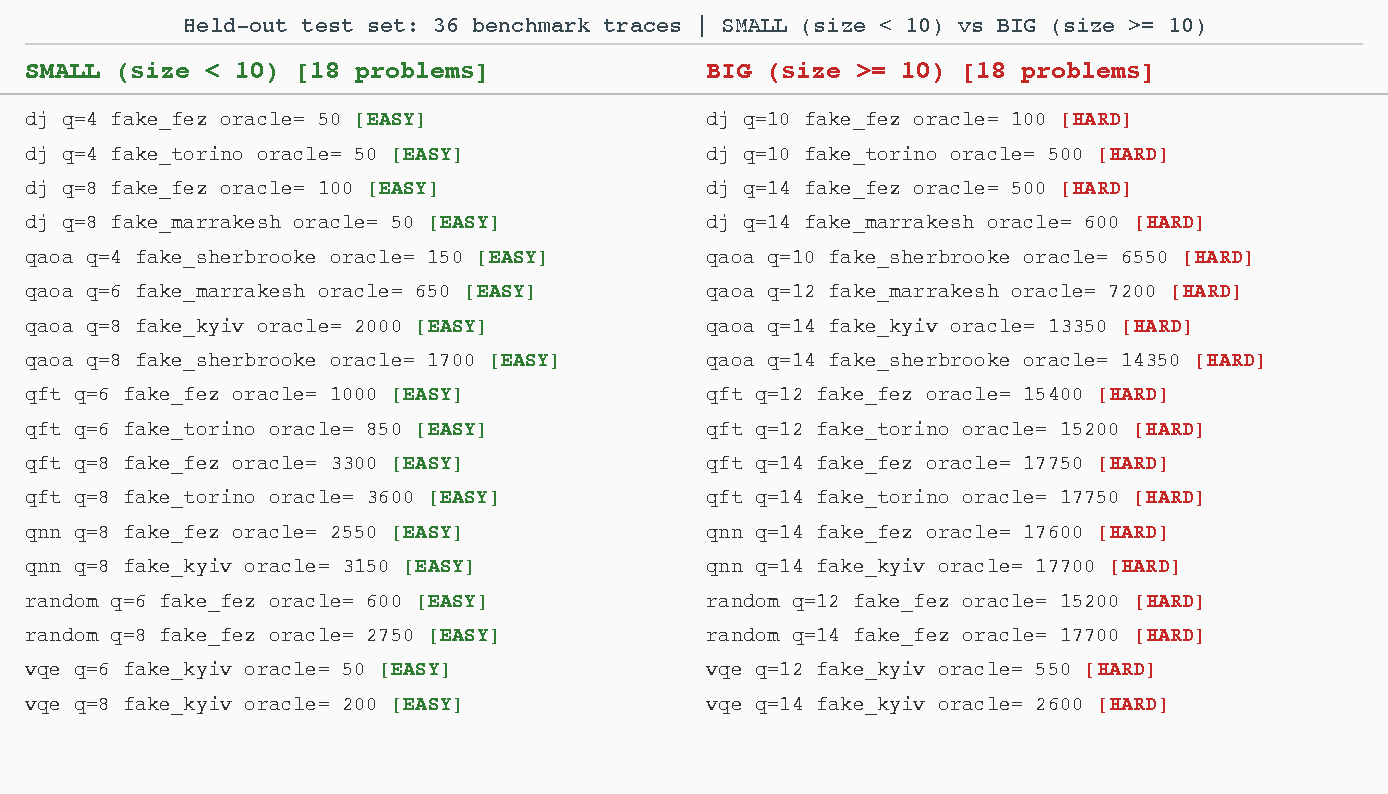
\includegraphics[width=0.95\textwidth]{problem_overview.pdf}
\caption{The 36 held-out benchmark traces (test set), grouped by circuit family,
size, backend, and a-posteriori Oracle shot count. These traces are never seen
during training.}
\label{fig:overview}
\end{figure}

A practical challenge is the heavy skew of the dataset toward ``easy'' instances
that converge with few shots. We address this with a configurable training
distribution (\emph{AgentType}): the \textsc{generic} agent studied here trains
on a balanced 50/50 mix of easy ($n<10$) and hard ($n\ge10$) problems, so it is
exposed to the full spectrum of convergence behaviours.

\section{Development and Experimental Setup}
\label{sec:setup}

\paragraph{Implementation.} The system is implemented in Python~3.12. The agent
and network use PyTorch~\cite{paszke2019pytorch}; the environment implements the
OpenAI Gym interface~\cite{brockman2016gym}; QSimBench supplies the circuit
traces and noise profiles. The full source code, oracle cache, and evaluation
scripts accompany this paper.

\paragraph{Training regimen.} Each agent is trained from scratch with a fixed
random seed for reproducibility. Validation for model selection uses a held-out
$20\%$ split of the training pool (disjoint from the 36 test traces). Starting
from a warm-up phase, the best model is checkpointed every $100$ episodes by
lowest validation Mean Absolute Error (MAE), with early stopping (patience $5$).

\paragraph{Model selection: how long to train?} An exploratory $10{,}000$-episode
run revealed three regimes. (i)~An initial \emph{stabilisation} phase in which
the agent adopts a conservative ``stop early'' baseline; the training MAE remains
high. (ii)~A \emph{breakthrough} around episodes $2{,}000$--$3{,}000$, where the
MAE drops sharply (by over $35\%$) as the agent learns circuit-specific stopping
behaviour, accompanied by increased reward variance. (iii)~An \emph{overfitting}
regime beyond $\sim$$3{,}000$ episodes, where the MAE plateaus while variance
keeps growing and the agent increasingly defaults to hyper-conservative
maximum-budget stops on ambiguous instances. We therefore train the production
agent for $3{,}000$ episodes, the empirical sweet spot between underfitting and
overfitting.

\paragraph{Evaluation protocol.} The selected agent is evaluated on the 36
held-out traces with a deterministic policy. To capture the stochasticity of
quantum sampling we run a \emph{multi-run} evaluation: the agent is replayed $N$
times per trace, and we report, per problem, the mean and standard deviation of
the shots used and of the resulting deviation from the Oracle. The headline
metric is the absolute deviation $|n_{\text{agent}}-n^{\star}|$ in shots; we also
report it as a percentage of the budget $\mathcal{B}$.

\section{Results}
\label{sec:results}

\subsection{Training Dynamics and Policy Alignment}

Figure~\ref{fig:dashboard} summarises the training and evaluation of the
$3{,}000$-episode \textsc{generic} agent. The reward moving average stabilises
quickly while the MAE undergoes the sharp breakthrough decline described above,
confirming that the learning is productive rather than a mere reward artefact.
Because outcomes are stochastic and the test circuits are unseen, the agent
cannot memorise a scalar shot count; to stop well it must interpret the dynamic
state features -- chiefly entropy, rate of change, and progress -- to locate the
point of stability.

\begin{figure}[t]
\centering
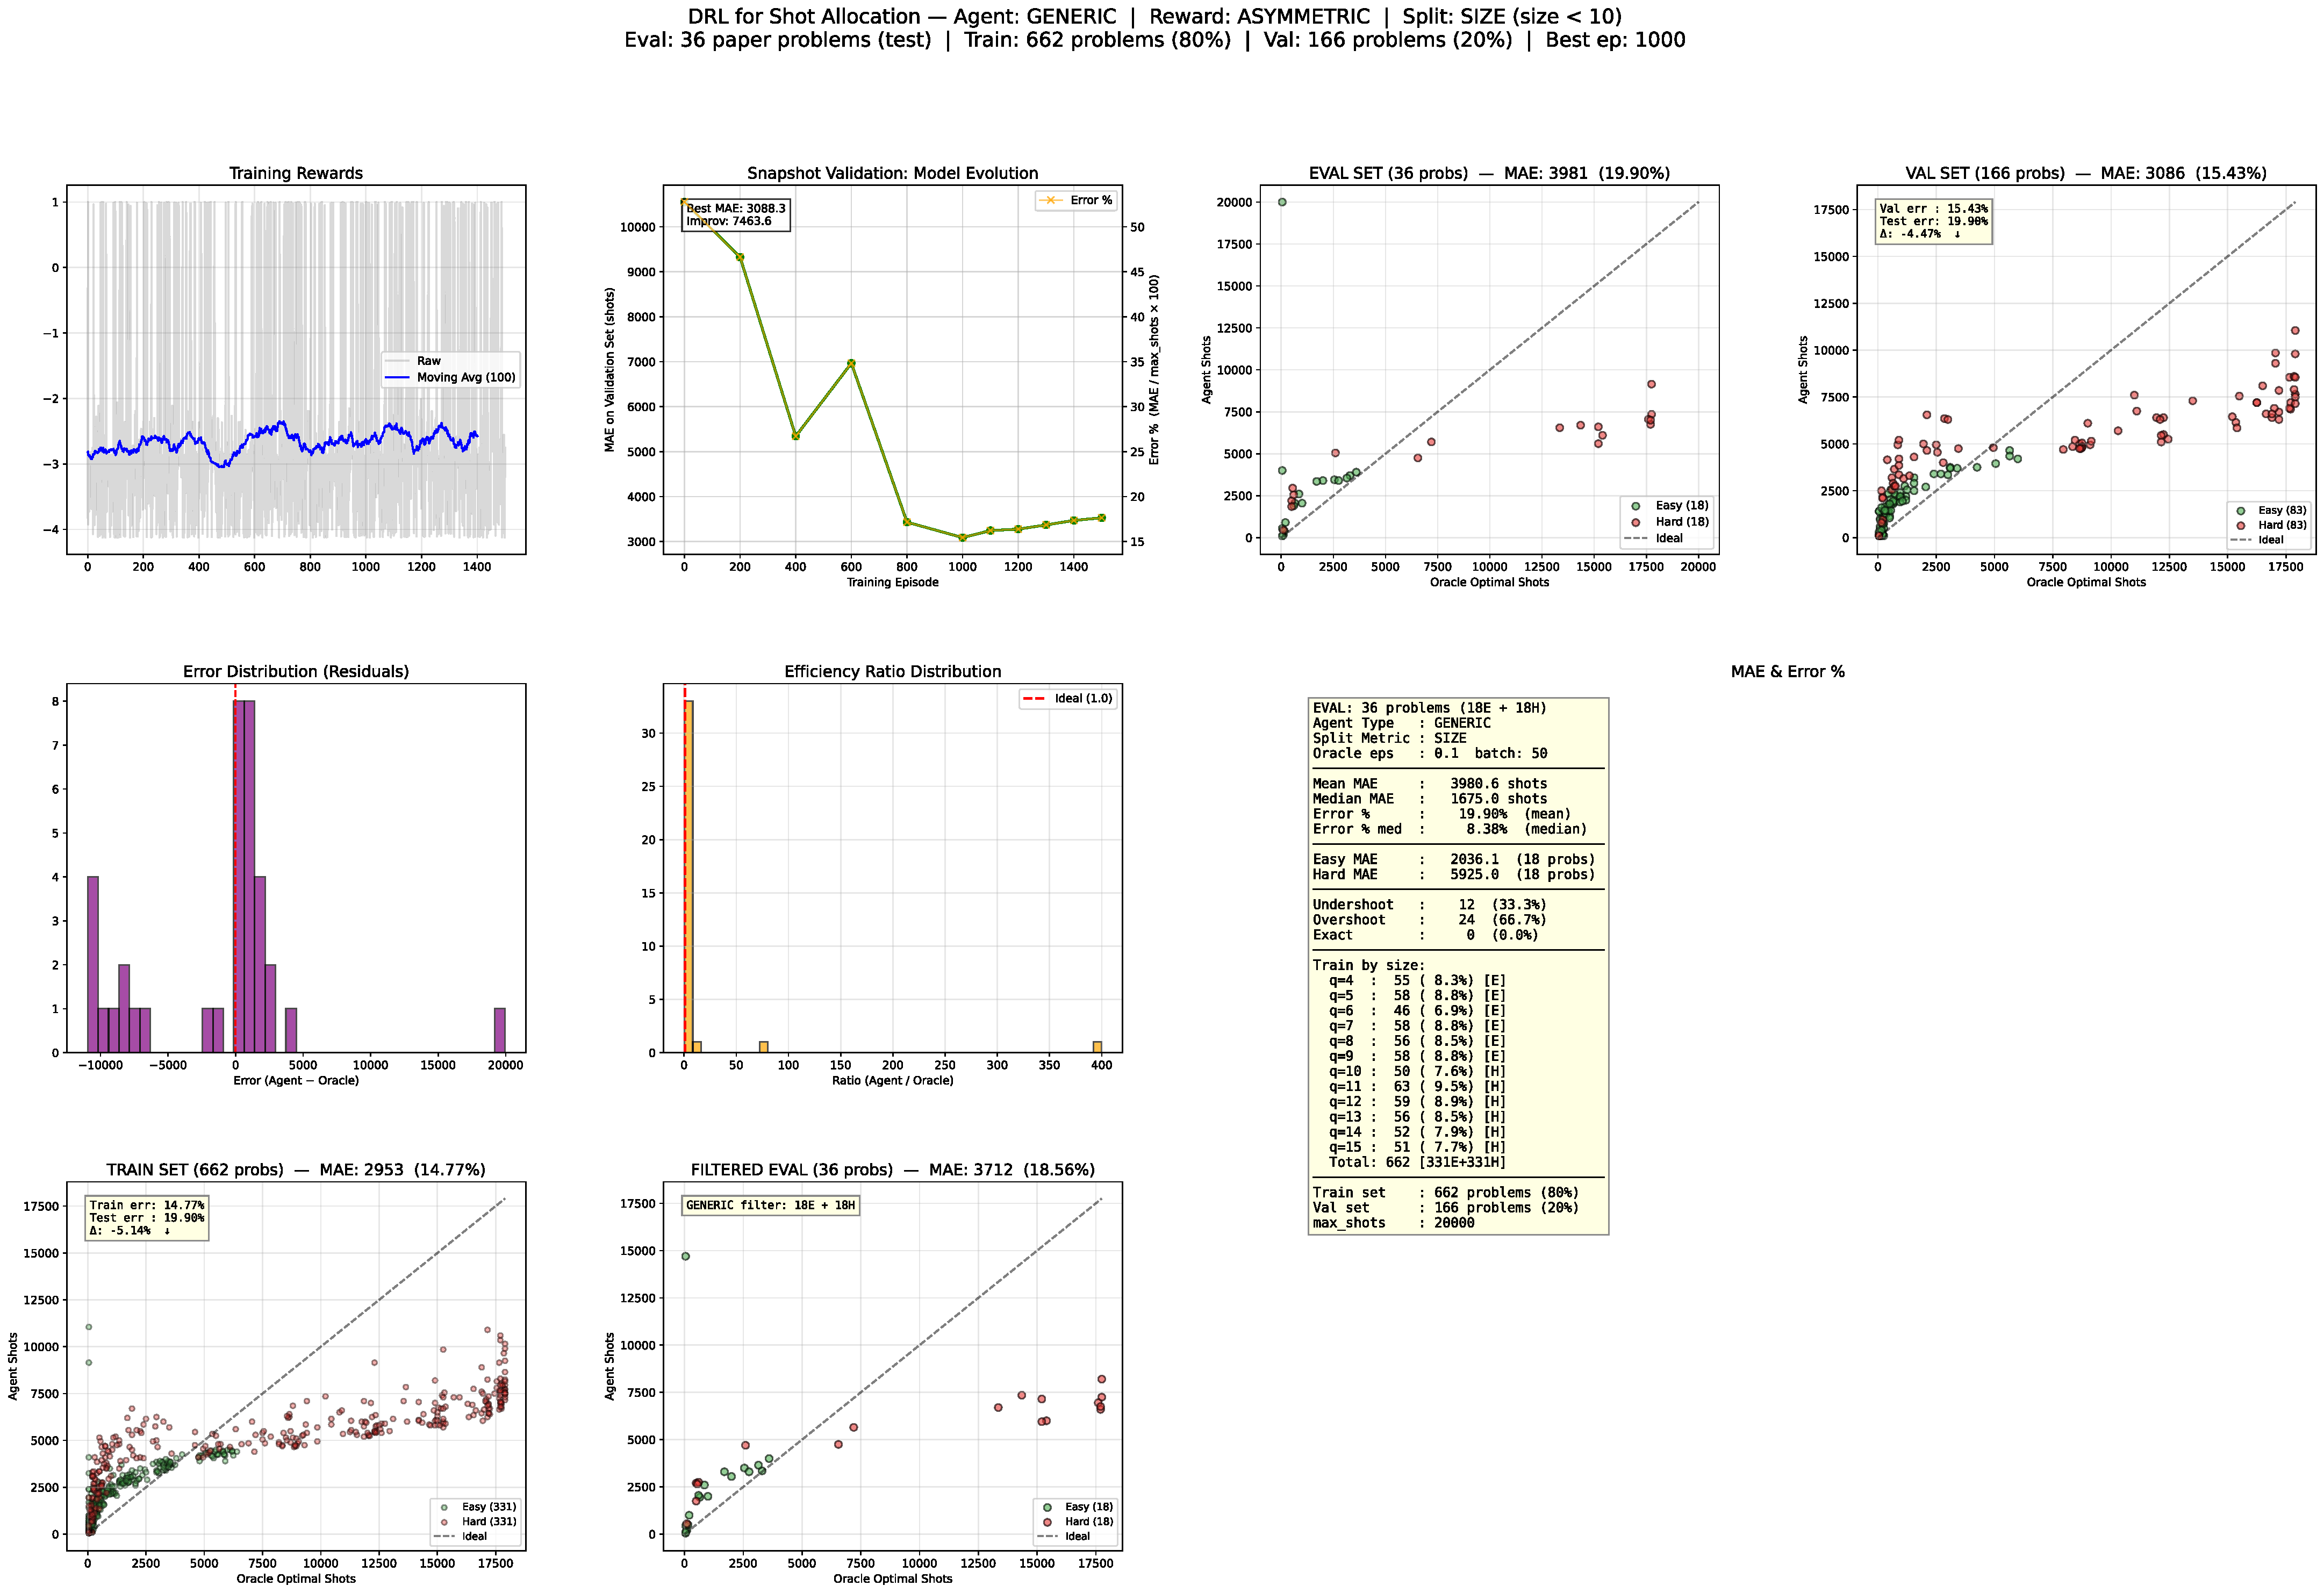
\includegraphics[width=\textwidth]{dashboard-generic.pdf}
\caption{Training and evaluation dashboard for the $3{,}000$-episode
\textsc{generic} agent: episodic reward and MAE during training, agent-vs-Oracle
policy alignment, and the distribution of stopping errors.}
\label{fig:dashboard}
\end{figure}

Figure~\ref{fig:scatter} plots, for each held-out trace, the shots chosen by the
agent against the Oracle optimum. Points on the diagonal denote perfect stops,
points above denote (safe) overshooting, and points below denote (risky)
undershooting. The agent tracks the Oracle well on easy and moderate instances;
on the hardest instances, where the Oracle approaches the budget, it tends to
stop conservatively before the optimum, the main residual source of error.

\begin{figure}[t]
\centering
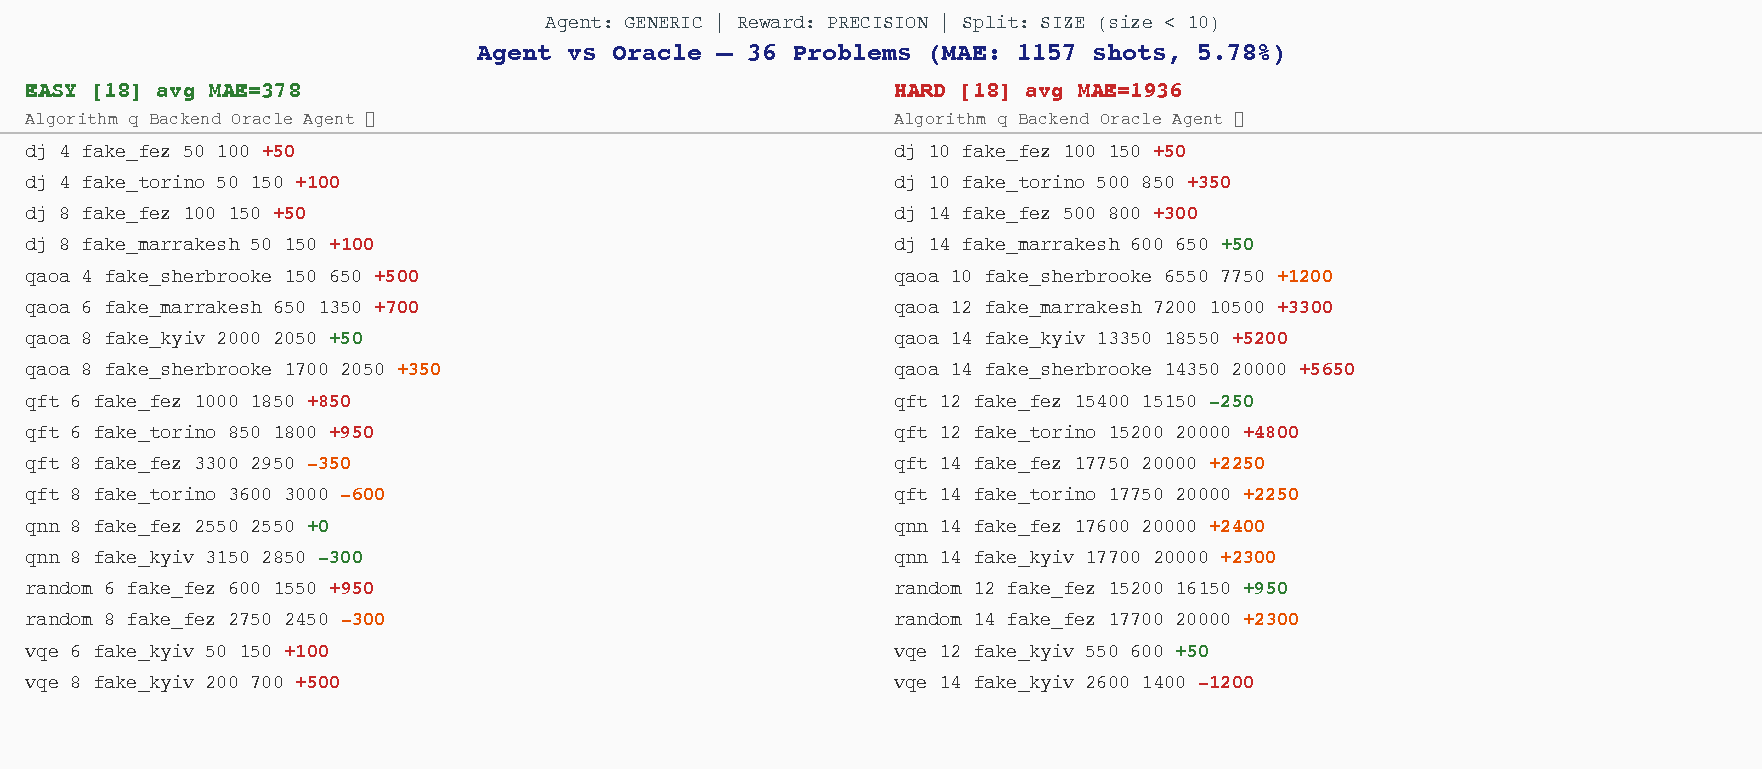
\includegraphics[width=0.85\textwidth]{agent_vs_oracle-generic-all36.pdf}
\caption{Agent policy vs.\ Oracle on the 36 held-out traces. The dashed line is
the perfect policy $y=x$.}
\label{fig:scatter}
\end{figure}

\subsection{Comparison with the State of the Art}

We compare the learned policy against five reference methods on the identical 36
traces at $\delta=0.10$: the three best online \textsc{IncrementalExecution}
configurations (\mbox{Inc-TVD}, \mbox{Inc-Hell}, \mbox{Inc-JS}) and the two
a-priori bounds (Weissman, Hoeffding)~\cite{bisicchia2026shots}. The aggregate
mean absolute deviation from the Oracle is reported in
Table~\ref{tab:aggregate}, and the full per-trace breakdown in
Tables~\ref{tab:pertrace-small}--\ref{tab:pertrace-large}.

\input{tables_generated}

Two findings stand out. First, the learned agent is overwhelmingly more
efficient than the a-priori bounds: Weissman and Hoeffding overshoot the Oracle
by roughly two and seven \emph{orders of magnitude} respectively, because they
must hold for the worst case over all distributions, whereas the agent adapts to
the observed statistics. Second, the agent is competitive with the
divergence-based online policies -- in the same regime as \mbox{Inc-JS} and
\mbox{Inc-Hell} -- but does not yet match the strongest baseline,
\mbox{Inc-TVD}, which was selected from an exhaustive grid of hand-tuned
configurations specifically for this metric. The agent achieves comparable
behaviour \emph{without} any hand-crafted stopping rule, learning the stopping
logic purely from data.

\medskip
\noindent\textit{Note on reproducibility of the reported numbers.} The DRL
columns in Tables~\ref{tab:aggregate}--\ref{tab:pertrace-large} are produced by
the script \texttt{make\_tables.py}, which merges the agent's multi-run
evaluation with the reference values. The values shown correspond to the current
single-run evaluation; the camera-ready version will report the mean$\pm$std over
ten independent evaluation runs of the selected best agent, regenerated by the
same script.

\subsection{Discussion}

\paragraph{Strengths.} (i)~\emph{Black-box generality}: the policy is driven only
by observed outcome statistics, with no access to the circuit or noise model, and
generalises to circuit families held out from training. (ii)~\emph{Safety-first
behaviour}: the asymmetric reward yields error distributions that are right-skewed
(the agent prefers a few extra shots to a premature, invalid stop), which is the
desirable bias in a scientific setting. (iii)~\emph{Modularity}: since the policy
is learned from the Oracle's signal rather than hard-coded, swapping the Oracle's
divergence (TVD $\to$ Hellinger/JS) only requires retraining, not redesign.

\paragraph{Limitations.} The agent does not yet outperform the best online
heuristic, and its dominant error mode is conservative \emph{undershooting on the
hardest, near-budget circuits}, where the dynamic signals are weakest and the
correct stop lies far into the budget. Prolonged training induces the opposite
pathology -- hyper-conservative maximum-budget stops on a few ambiguous easy
instances -- consistent with overfitting to the asymmetric reward. Both point to
the reward shaping and the hard-instance coverage of the training distribution as
the primary levers for improvement.

\section{Threats to Validity}
\label{sec:threats}

\emph{Construct validity.} We score against an a-posteriori Oracle rather than the
inaccessible true distribution; this is the same principled reference used by the
state of the art~\cite{bisicchia2026shots}, and we use the identical $\delta$,
budget, and batch size for comparability. \emph{Internal validity.} Quantum
sampling is stochastic; we mitigate run-to-run variance through multi-run
evaluation and fixed seeds. \emph{External validity.} Experiments use IBM noisy
\emph{simulators} from QSimBench rather than live hardware, and target static,
non-variational circuits; transfer to real devices and to variational workloads
remains future work.

\section{Conclusion and Future Work}
\label{sec:conclusion}

We presented a Deep Reinforcement Learning approach to adaptive shot allocation
that learns, under a strict black-box assumption, when to stop sampling a quantum
circuit. Framed as a Markov Decision Process with an eight-feature state and an
asymmetric, safety-oriented reward, a Deep Q-Network learns a stopping policy
that generalises to unseen circuit families, dramatically outperforms a-priori
concentration bounds, and is competitive with purpose-built online heuristics --
all without encoding any explicit convergence test. This establishes that
black-box shot allocation is learnable.

Future work targets the remaining gap with the best online policy: refining the
reward to better handle near-budget hard instances, enriching the state with
additional convergence descriptors, exploring distributional and double DQN
variants, evaluating mean$\pm$std over ten runs of the selected agent, and
ultimately validating on live quantum hardware and extending the formulation
toward variational workloads.

\subsubsection*{Acknowledgements.} This work builds on the QSimBench benchmark
and the \textsc{IncrementalExecution} framework developed at the University of
Pisa.

\bibliographystyle{splncs04}
\bibliography{references}

\end{document}
